\documentclass[compress]{beamer}
\usepackage{ifthen,verbatim}

\newcommand{\isnote}{}
\xdefinecolor{lightyellow}{rgb}{1.,1.,0.25}
\xdefinecolor{darkblue}{rgb}{0.1,0.1,0.7}

%% Uncomment this to get annotations
%% \def\notes{\addtocounter{page}{-1}
%%            \renewcommand{\isnote}{*}
%% 	   \beamertemplateshadingbackground{lightyellow}{white}
%%            \begin{frame}
%%            \frametitle{Notes for the previous page (page \insertpagenumber)}
%%            \itemize}
%% \def\endnotes{\enditemize
%% 	      \end{frame}
%%               \beamertemplateshadingbackground{white}{white}
%%               \renewcommand{\isnote}{}}

%% Uncomment this to not get annotations
\def\notes{\comment}
\def\endnotes{\endcomment}

\setbeamertemplate{navigation symbols}{}
\setbeamertemplate{headline}{\mbox{ } \hfill
\begin{minipage}{5.5 cm}
\vspace{-0.75 cm} \small
\end{minipage} \hfill
\begin{minipage}{4.5 cm}
\vspace{-0.75 cm} \small
\begin{flushright}
\ifthenelse{\equal{\insertpagenumber}{1}}{}{Jim Pivarski \hspace{0.2 cm} \insertpagenumber\isnote/\pageref{numpages}}
\end{flushright}
\end{minipage}\mbox{\hspace{0.2 cm}}\includegraphics[height=1 cm]{../cmslogo} \hspace{0.1 cm} \includegraphics[height=1 cm]{../tamulogo} \hspace{0.01 cm} \vspace{-1.05 cm}}

\begin{document}
\begin{frame}
\vfill
\begin{center}
\textcolor{darkblue}{\Large Muon Jets Analysis}

\vfill
\begin{columns}
\column{0.3\linewidth}
\begin{center}
\large
Jim Pivarski
\end{center}
\end{columns}

\begin{columns}
\column{0.3\linewidth}
\begin{center}
\scriptsize
{\it Texas A\&M University}
\end{center}
\end{columns}

\vfill
12 July, 2010

\end{center}
\end{frame}

%% \begin{notes}
%% \item This is the annotated version of my talk.
%% \item If you want the version that I am presenting, download the one
%% labeled ``slides'' on Indico (or just ignore these yellow pages).
%% \item The annotated version is provided for extra detail and a written
%% record of comments that I intend to make orally.
%% \item Yellow notes refer to the content on the {\it previous} page.
%% \item All other slides are identical for the two versions.
%% \end{notes}

\small

\begin{frame}
\frametitle{Motivation 1: dark matter}
\begin{enumerate}
\item PAMELA expreiment saw an excess of high-energy positrons in primary cosmic rays
\begin{itemize}
\item cannot be galactic modelling (even pushing parameters beyond the limit can't make the spectrum {\it increase} with energy
\item could be as-yet unknown young pulsars near Earth
\item could be decay products of WIMP-WIMP annihilation, except the cross-section is too high
\end{itemize}

\item Adding a long-range force that couples strongly to WIMPs, weakly to SM, could explain it:
\begin{itemize}
\item ``dark photon,'' a $\sim$1~GeV boson, acts as a long-range force attracting slow-moving WIMPs, more likely to collide
\item doesn't change the ``WIMP miracle'' in the early universe (fast-moving WIMPs)
\item 1~GeV boson is kinematically constrained to decay into $e^+e^-$,
  $\mu^+\mu^-$, $\pi\pi\pi$, all of which would eventually give an
  excess of positrons (observed) and not antiprotons (not observed)
\end{itemize}

\item In the LHC, this would show up as a low-mass but high-momentum
  resonance (it must be produced in top-down decays, since it has not
  been discovered already in low-energy collisions)
\end{enumerate}
\end{frame}

\begin{frame}
\frametitle{Motivation 2+}
\begin{itemize}
\item NMSSM $h \to aa \to 4\mu$: unexplored region of parameter space that could be hiding the Higgs boson
\begin{enumerate}
\item electroweak precision fits want a light Higgs ($\sim$100~GeV),
  but limits {\it assuming SM-like branching fractions} are at 114~GeV
\item not a contradiction yet, but some $2\sigma$-ish tension in the fit
\item the Higgs boson responsible for electroweak symmetry breaking
  must have partial widths proportional to mass-squared of the decay
  products ($\Gamma_{SM}$)
\item but if there are multiple Higgses ($h$, $a$, and others), and
  Higgs-to-Higgs partial widths are large ($\Gamma_{H-H}$), then
  SM-like branching fractions would be smaller than we're assuming:
  $\mathcal{B}_X = \Gamma_X / \sum_i \Gamma_i$
\item we found a region of NMSSM parameter space in which $\mathcal{B}
  \to aa$ is high ($\sim$100\%), $a \to \mu\mu$, so a 100~GeV $h$
  would disappear into $4\mu$ rather than SM-like modes
\end{enumerate}

\item Generic: this topology wouldn't necessarily be caught by other
  analyses, though our detector should be very sensitive to it
\begin{itemize}
\item theories seem to be satisfied with a wide variety of things
  thrown into this hidden sector: we should look
\end{itemize}
\end{itemize}
\end{frame}

\begin{frame}
\frametitle{Signature}
\begin{itemize}
\item Most generally, at least two muons with high momentum (comes
  from a top-down decay) and low mass

\item There may be other light resonances in the sector: this can lead
  to more than two muons in a small cone: $pp \to X \mbox{ light} \to
  \mbox{lightest}\mbox{ lightest} \to >2 \mu$

\item There may be other heavy resonances in the sector: this can lead
  to multiple pairs/groups of muons in the same event: $pp \to X
  \mbox{ heavy} \to \mbox{light}\mbox{ light} \to 2\mu, 2\mu$

\item They may be accompanied by missing energy (WIMPs) or they may
  have highly displaced vertices (if they couple very weakly to the
  SM)
\end{itemize}

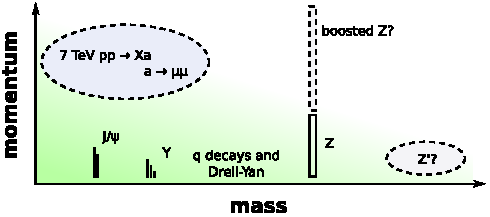
\includegraphics[height=3 cm]{where_we_live.pdf}
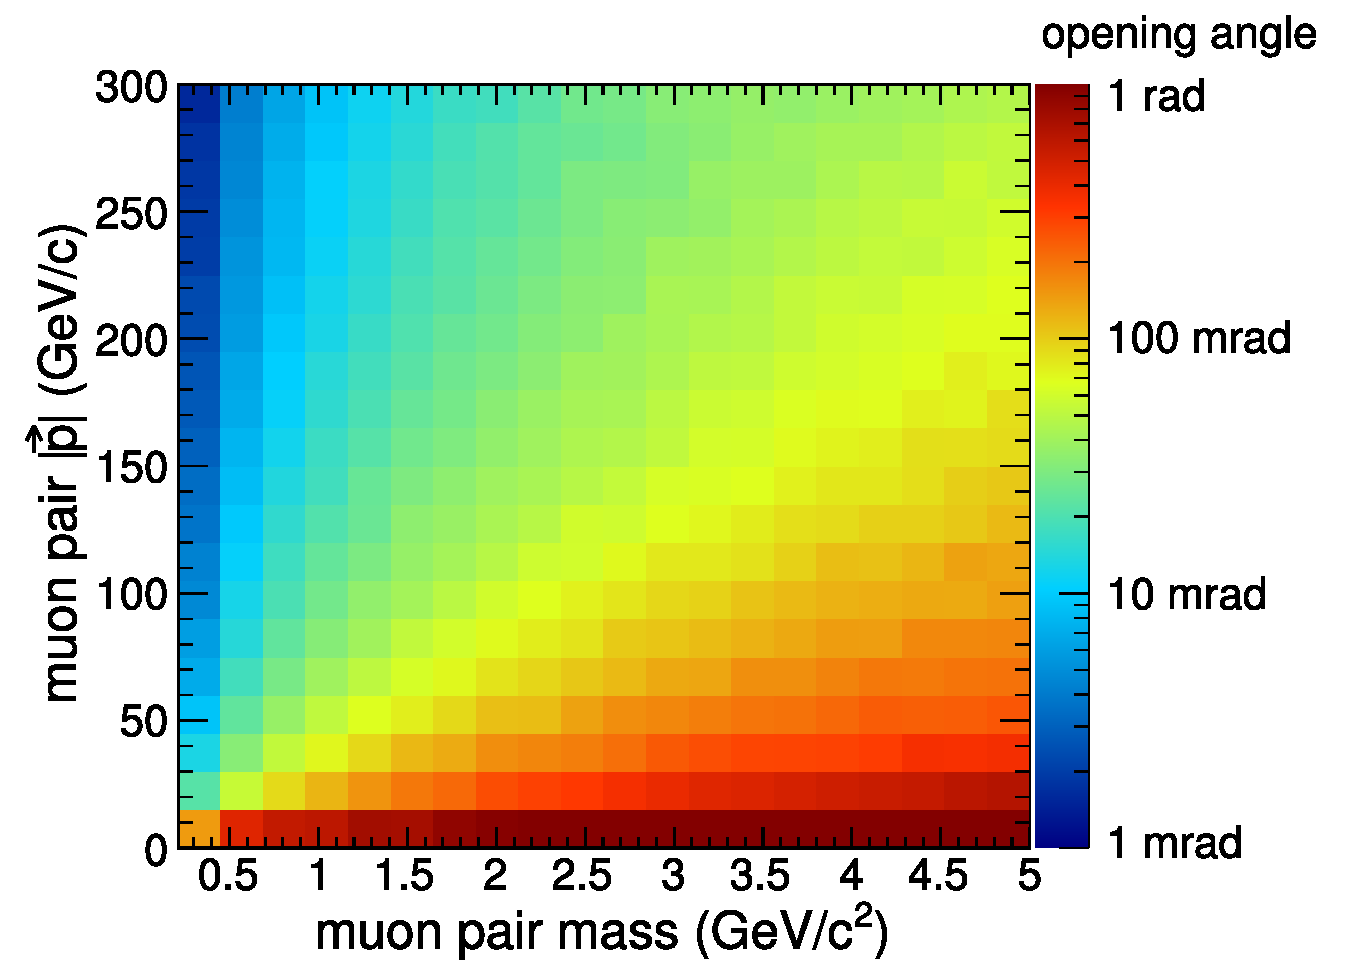
\includegraphics[height=3 cm]{openingangle_angle.pdf}
\end{frame}

\begin{frame}
\frametitle{Essence of the analysis}
\begin{itemize}
\item This is a search-and-discovery (or place limits); the important points are
\begin{itemize}
\item be general: cast a wide net so that we don't miss a discovery
\begin{itemize}
\item must identify signature-based variables and quote limits in
  those variables, so that they are applicable to many different
  theories: what variables identify this signature?
\end{itemize}

\item understand the backgrounds, so that we don't falsely claim a discovery
\begin{itemize}
\item must find variables in which the signature is clearly distinct from backgrounds
\item data-driven backgrounds estimates: can be estimated from
  variables that are nearly independent of one another
\end{itemize}
\end{itemize}
\end{itemize}
\end{frame}

\begin{frame}
\frametitle{What we know: backgrounds}

\begin{itemize}
\item From quick backgrounds studies (in April/May):
\begin{itemize}
\item 1~pb (target signal cross-section) is $\sim 10^3$ times smaller cross-section than background
\item single-``muon jet'' analysis should require $>$ 2 muons, high $p_T$
  cuts, and careful segment arbitration to suppress $pp \to X \mu$
\item multiple-``muon jet'' analysis with $>$ 1 jet is pretty safe,
  especially as a mass-peak search (e.g.\ NMSSM analysis)
\item isolation (defined properly for multi-muons) suppresses background by a factor of 10
\end{itemize}
\end{itemize}

\begin{columns}
\column{0.65\linewidth}
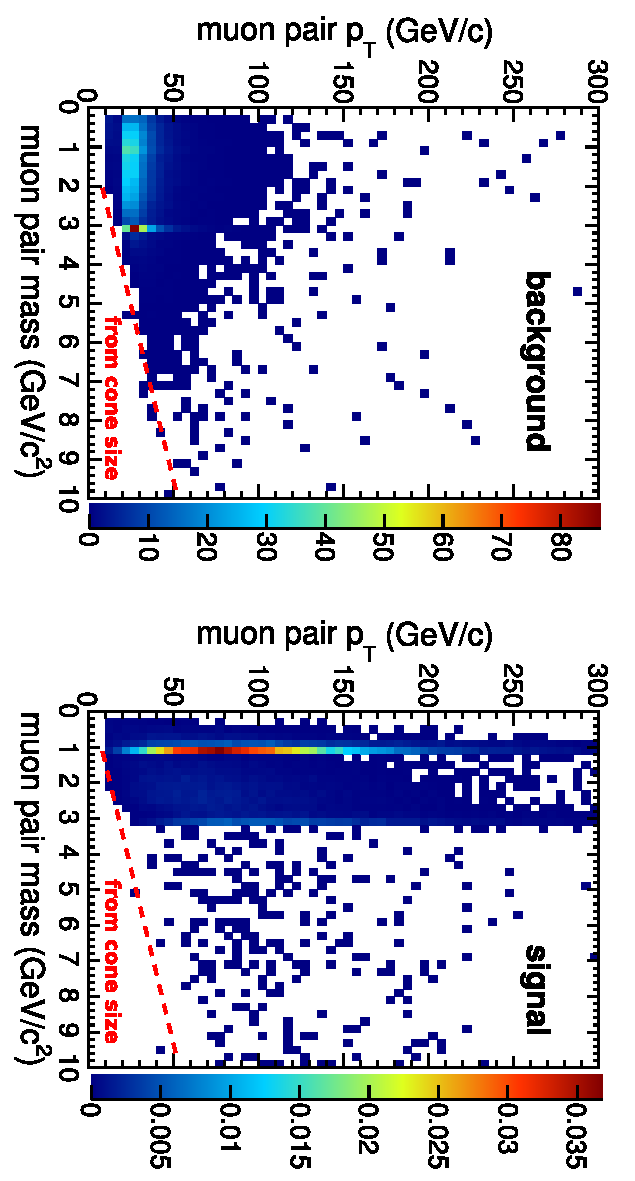
\includegraphics[height=\linewidth, angle=90]{backgrounds_basic.pdf}
\column{0.35\linewidth}
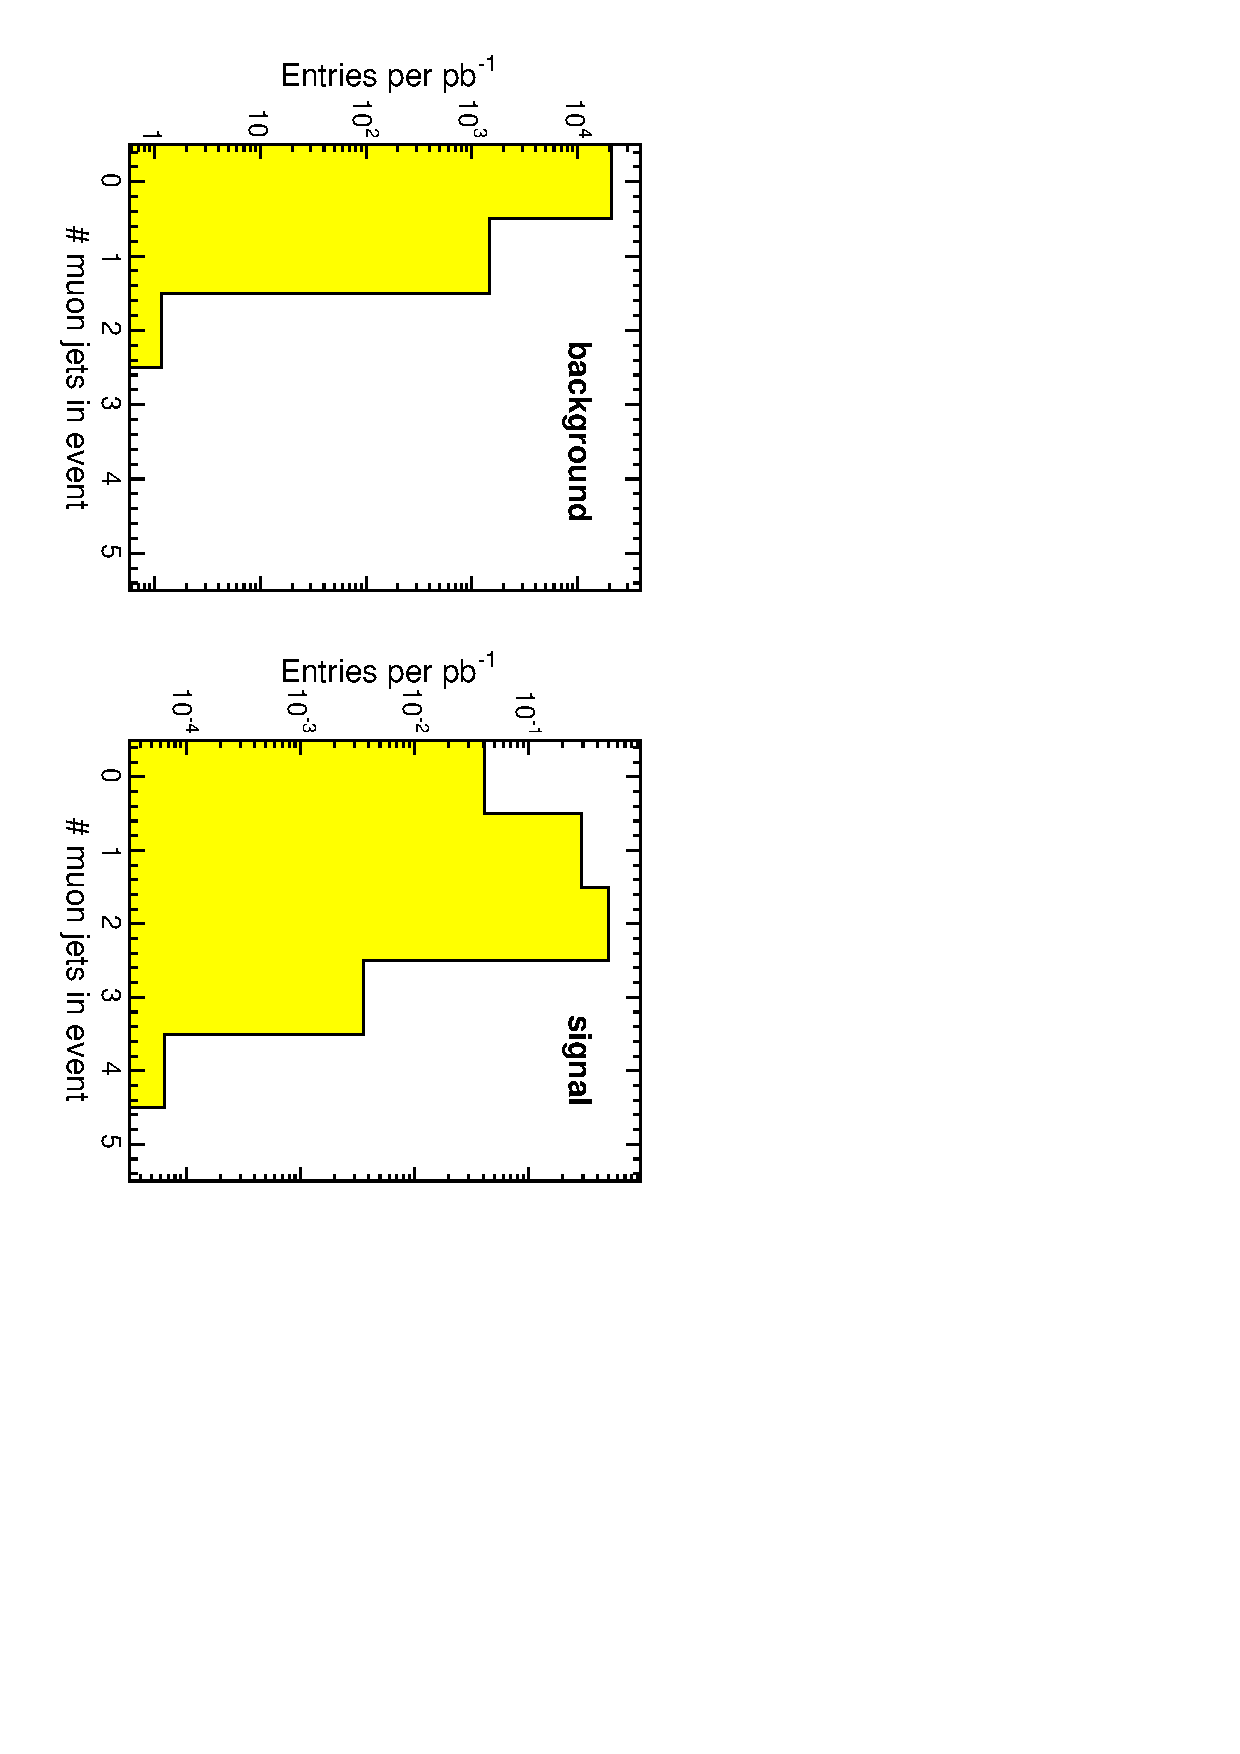
\includegraphics[height=\linewidth, angle=90]{backgrounds_jetsperevent.pdf}

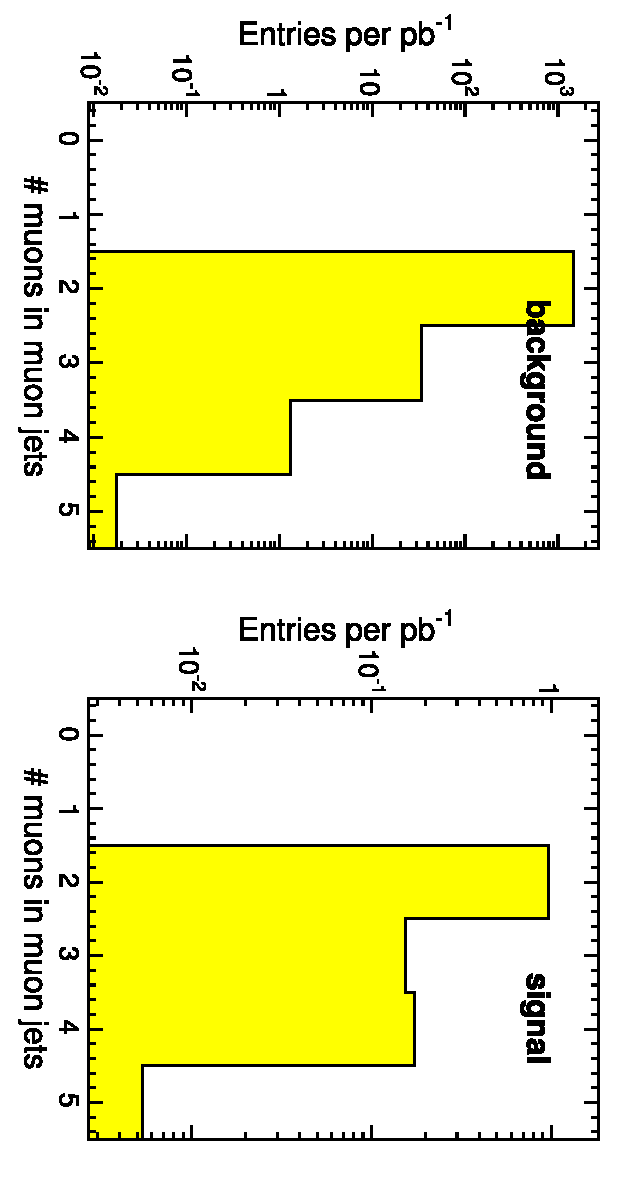
\includegraphics[height=\linewidth, angle=90]{backgrounds_muonsperjet.pdf}
\end{columns}
\end{frame}

\begin{frame}
\frametitle{What we know: reconstruction}

\vspace{1 cm}
\hfill 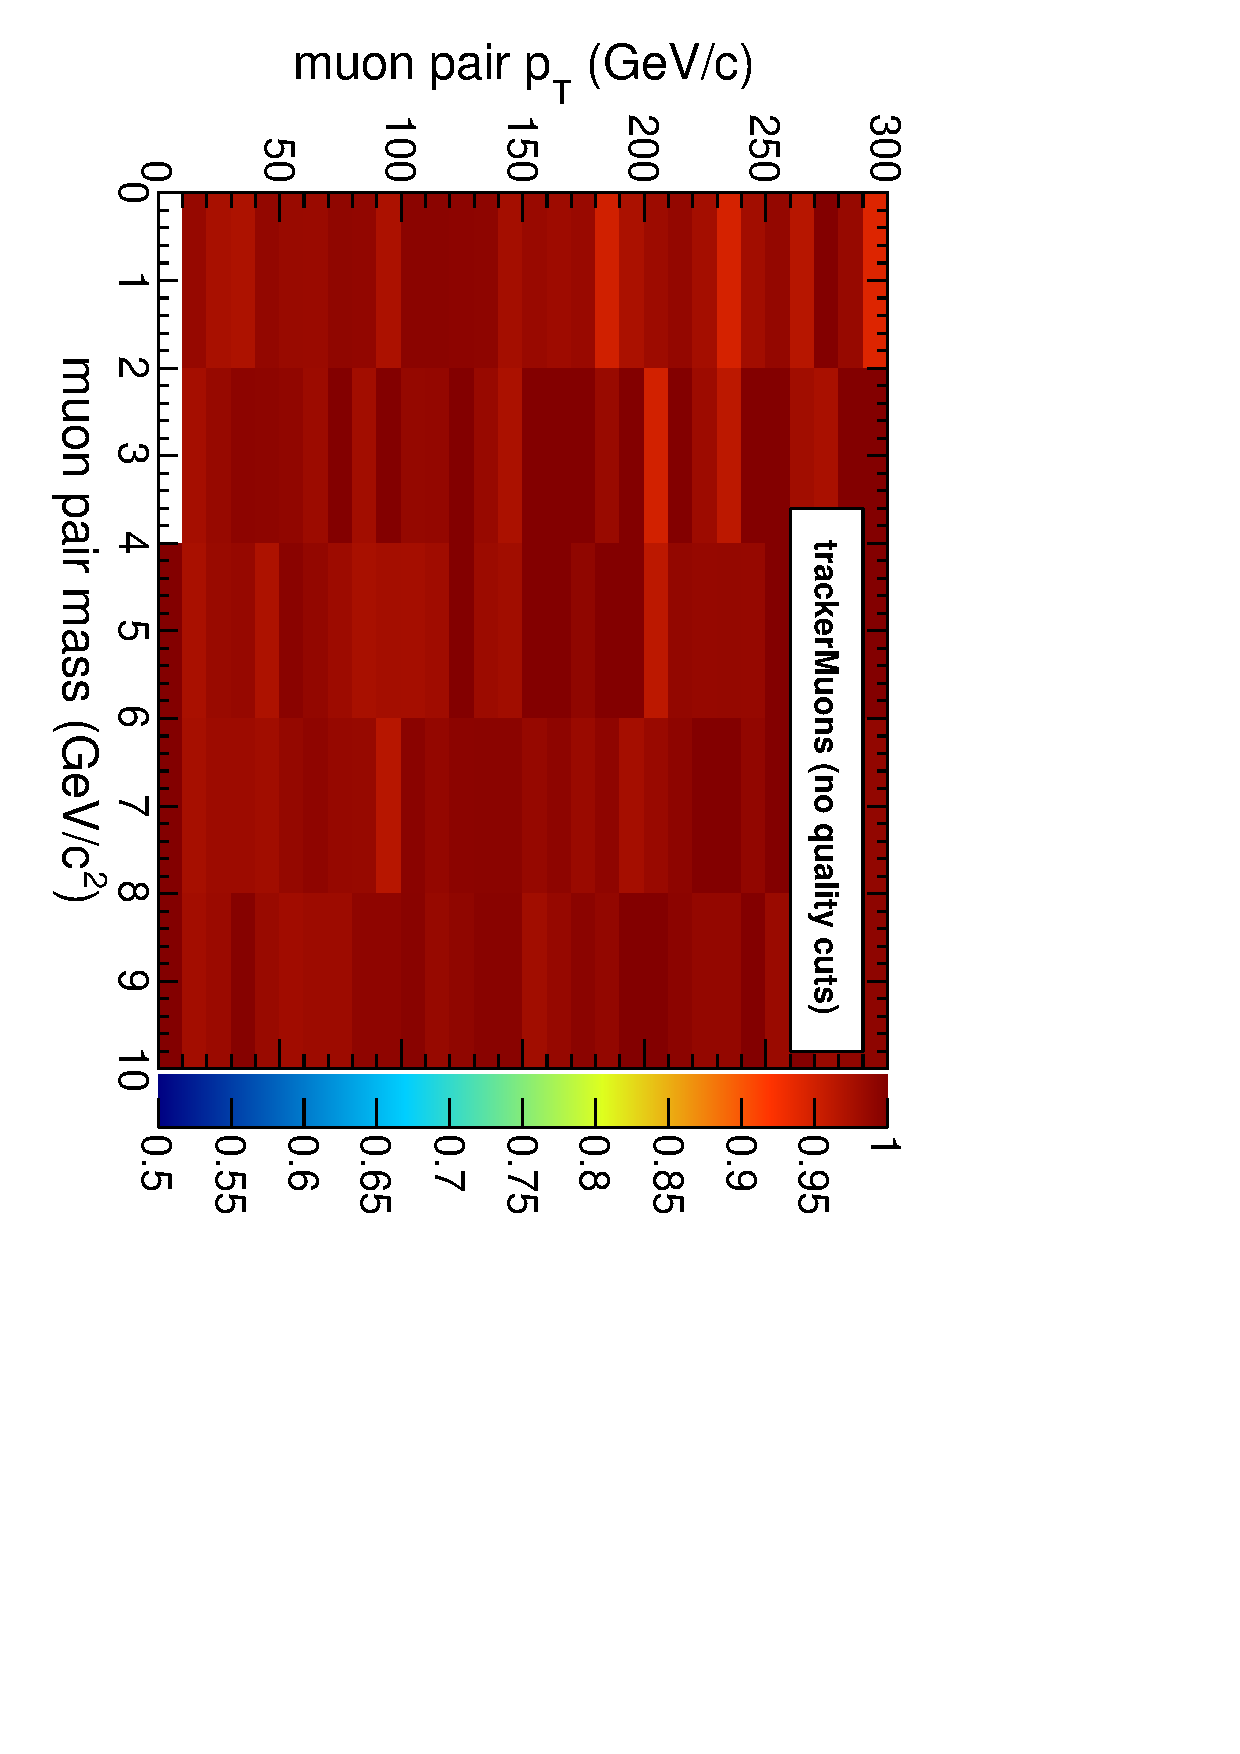
\includegraphics[height=0.5\linewidth, angle=90]{efficiency2d_tracker.pdf}

\vspace{-5 cm}
\begin{itemize}
\item Tracker muons (e.g.\ prev page) have high efficiency but high backgrounds
\begin{itemize}
\item backgrounds are higher \\ than they need to be \\ because multiple
  tracker \\ tracks can be associated \\ with the same segments
\item ``arbitration:'' assigning \\ each segment with exactly \\ one track,
  is provided by \\ several standard algorithms, \\ but they are ``greedy
  algorithms'' and therefore order-dependent (leading muon gets all of
  the best segments)
\item something that might not be appropriate: I have an idea for calculating a
  unique optimal arbitration (later slide), can check to see how close the standard
  algorithms get to optimal arbitration as a function of $\Delta R$
\end{itemize}
\end{itemize}
\end{frame}

\begin{frame}
\frametitle{What we know: reconstruction}

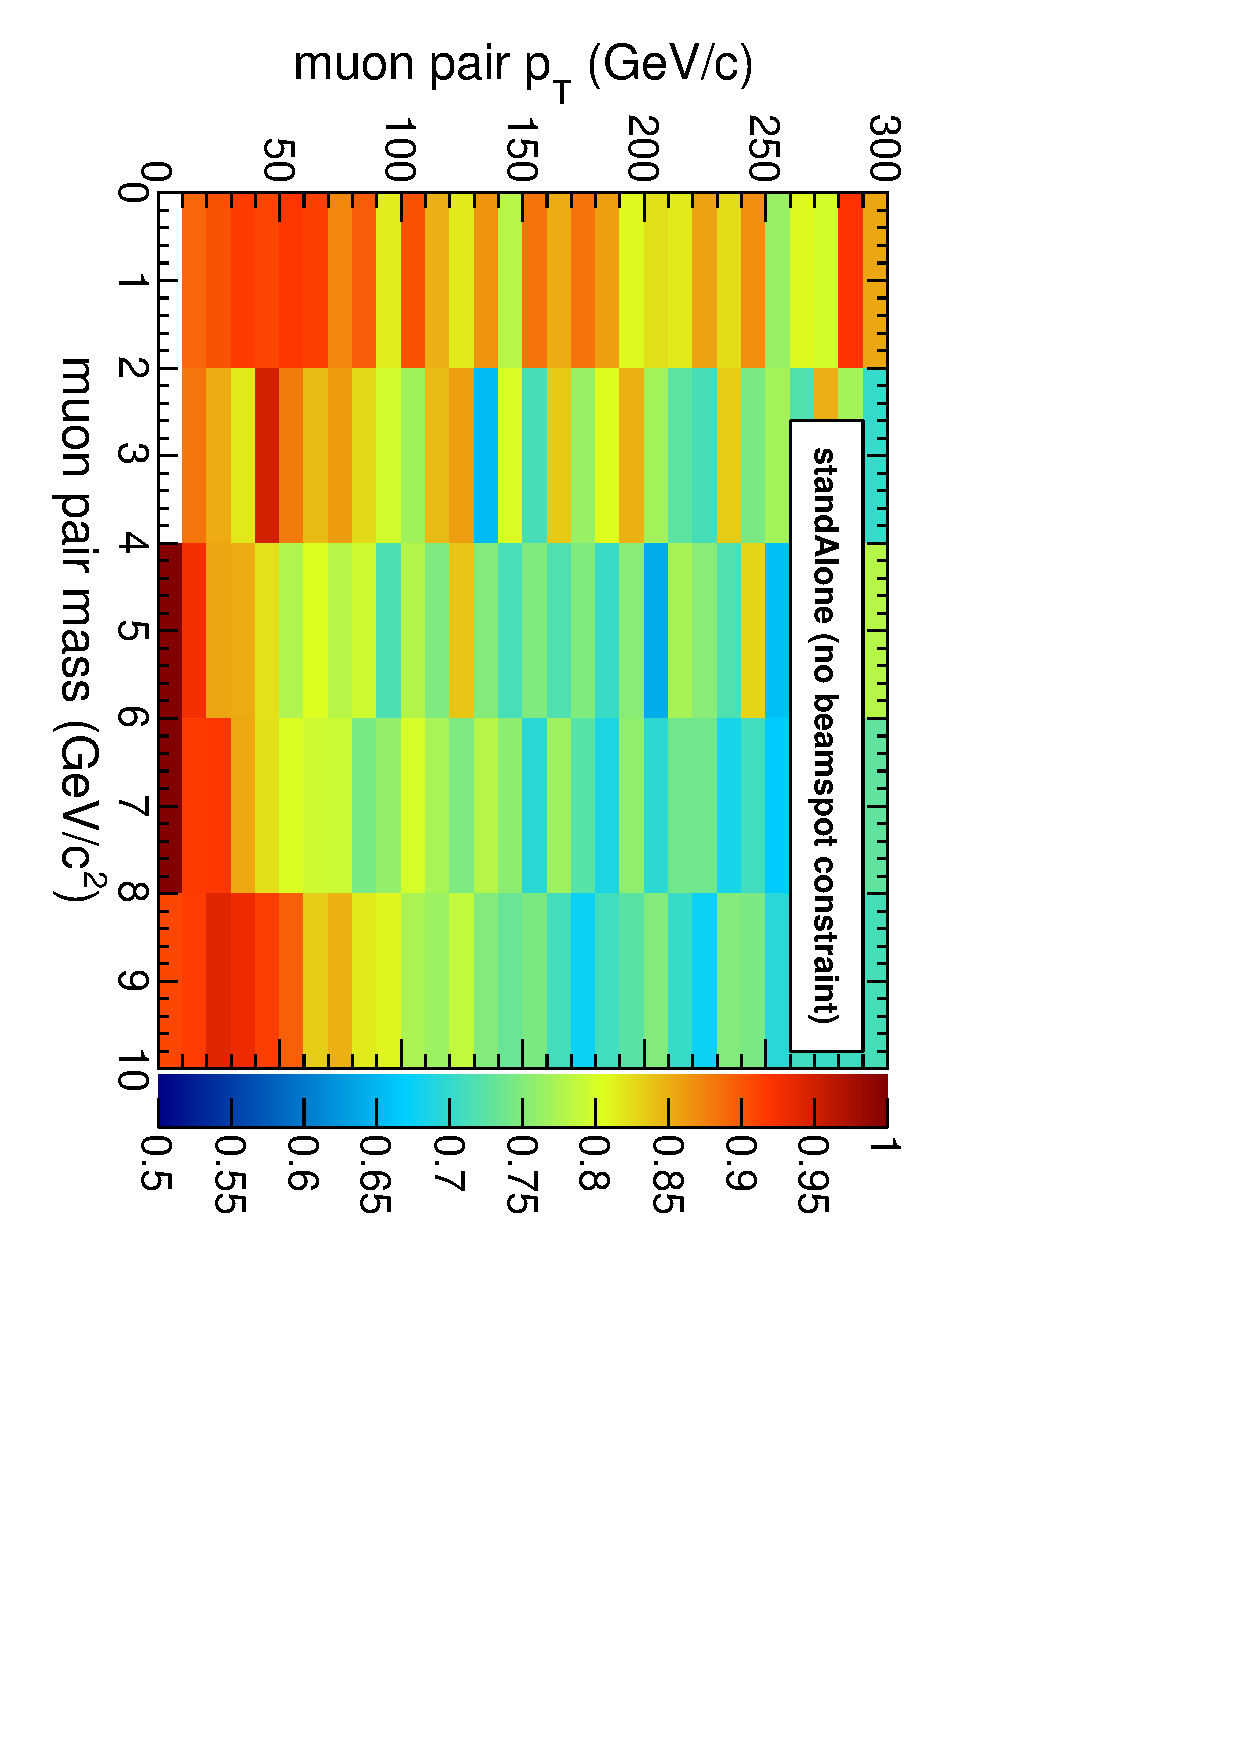
\includegraphics[height=0.5\linewidth, angle=90]{efficiency2d_stand.pdf}
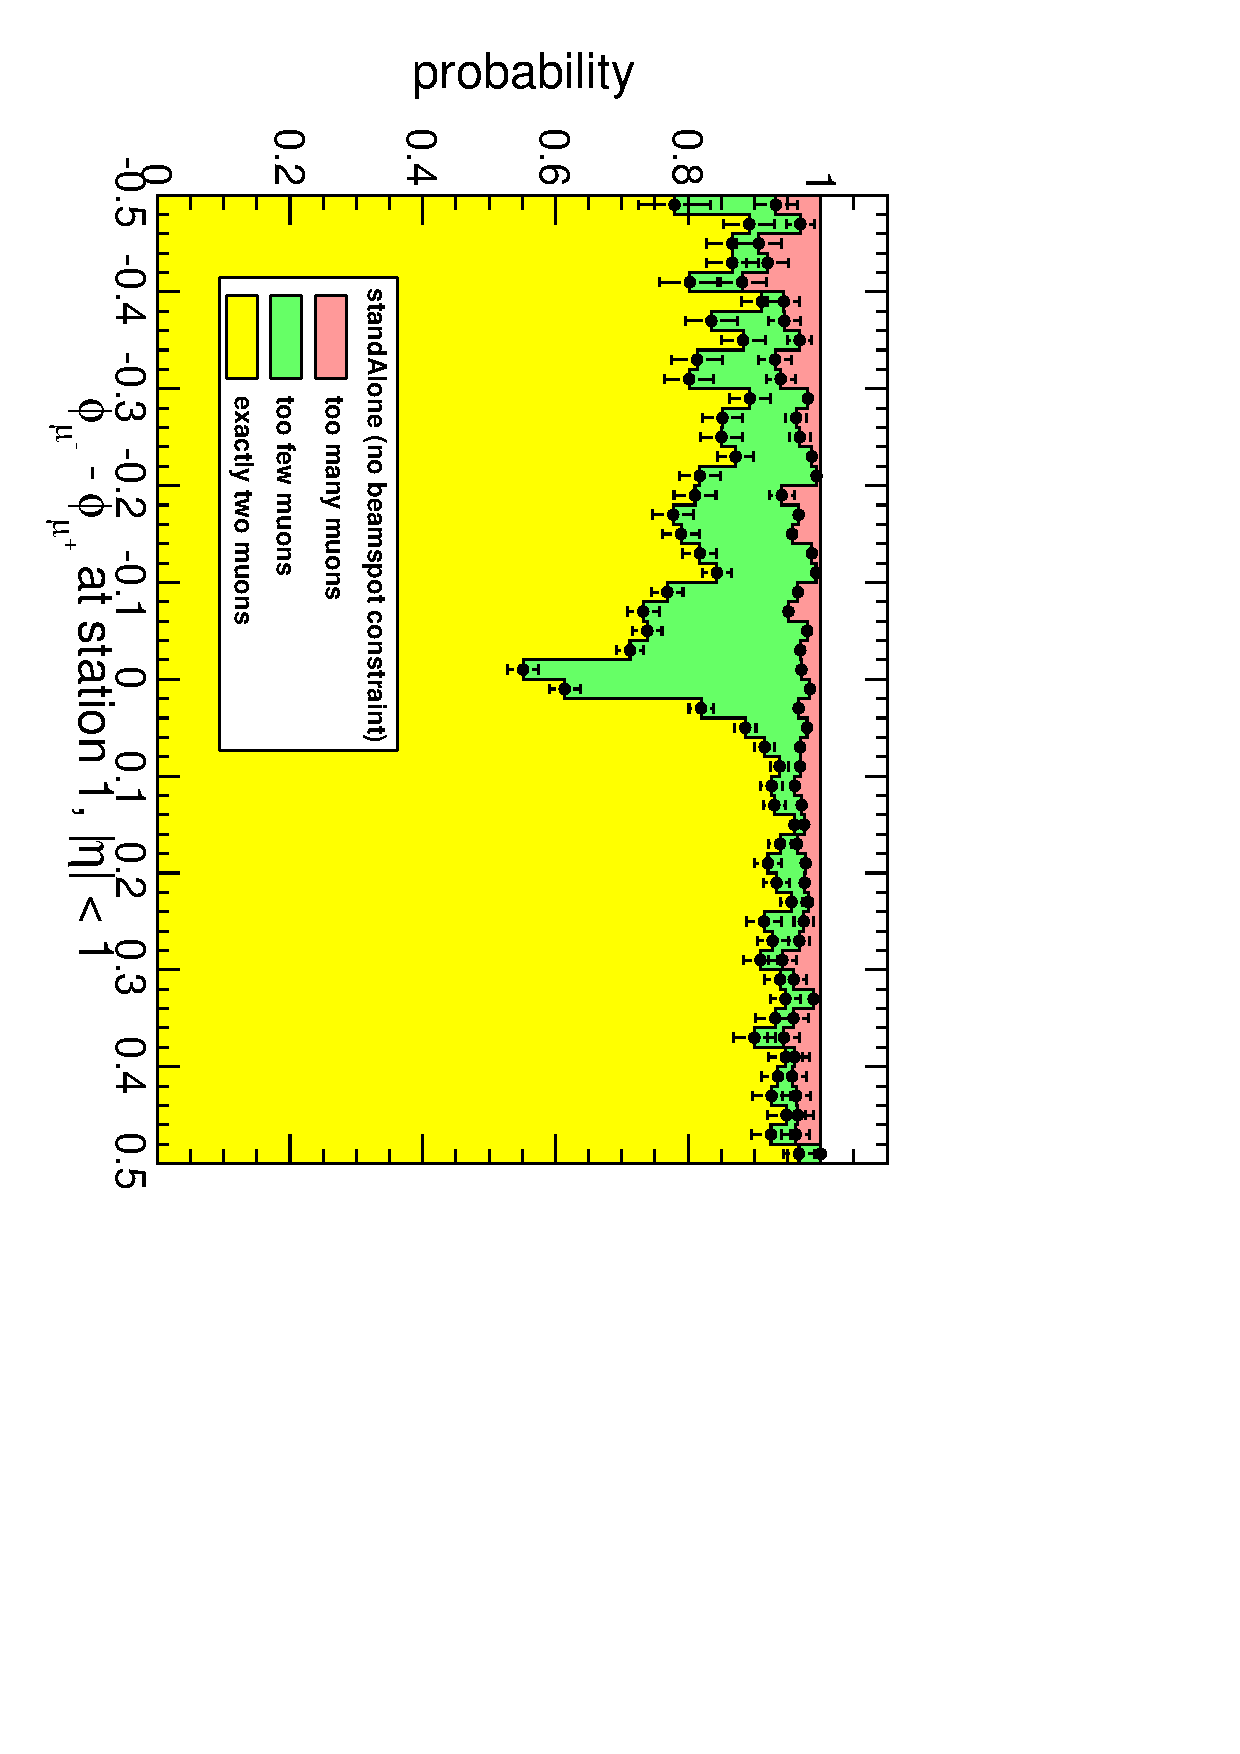
\includegraphics[height=0.5\linewidth, angle=90]{efficiency_standPhiDiff0.pdf}

\begin{itemize}
\item Stand-alone muons: low efficiency, especially when the two muons
  cross each other in the muon system
\begin{itemize}
\item appears to be a cut in the stand-alone muon finding
\end{itemize}
\item Global muons: built from stand-alone muons, so they should
  inherit this inefficiency
\item Something to try: the ``SET'' stand-alone algorithm under
  development by Ingo, Stoyan, and others
\end{itemize}
\end{frame}

\begin{frame}
\frametitle{Current status}
\begin{enumerate}
\item Pilot study, to know what to look for in general study \hfill \textcolor{darkblue}{done}
\item Building framework and datasets for general study \hfill \textcolor{darkblue}{99\% done}
\item Exploration of the datasets, figuring out which plots \hfill \textcolor{darkblue}{a little bit} \\ to put in a general analysis note
\item Systematically making all of the plots so that everything (all cuts, etc) is mutually consistent and can be repeated
\item Putting them into an analysis note
\item Doing the same with data, data/MC comparisons, another analysis note
\item Writing a paper\ldots
\end{enumerate}

\vfill
This means that I have no plots to show, but I can show a lot of the work that has been done:

\href{https://twiki.cern.ch/twiki/bin/view/CMS/ExoticaMuonJets}{\textcolor{blue}{https://twiki.cern.ch/twiki/bin/view/CMS/ExoticaMuonJets}}

(I've been filling this out like a lab notebook as I go along)
\end{frame}

\begin{frame}
\frametitle{Event samples}
\begin{itemize}
\item pat::Muon collections created from several sources:
\begin{itemize}
\item NormalMuons: the collection provided by the muon POG (the set of all globalMuons are a subset of this)
\item TrackerMuons: all muons that can be identified with the trackerMuons algorithm, no arbitration
\item TrackerMuonsConv: same with tracks produced using the exhaustive
  7-iteration tracking developed for $e^+e^-$ conversions, may extend
  the range of displaced-vertex searches
\item StandAloneDefault and StandAloneSET: stand-alone muons with the default and SET algorithms (no beamline constraint)
\end{itemize}

\item Very loose skim cut: $\ge 2$ muons in any collection

\item Carefully chosen reduced set of branches makes the above practical (all MET variables, trigger data, MC truth included)

\item Skims of all InclusiveMu5\_PtX

\item Example signal samples (extra-$\mathcal{U}(1)$ dark matter and NMSSM)

\item Many muon-jet guns, generated uniformly in resonance mass and
  momentum, some with large displace vertices, with \& w/o pile-up
\end{itemize}
\end{frame}

\begin{frame}
\frametitle{Software}
\begin{itemize}
\item Tools for gluing groups of muons together according to various
  criteria: $\Delta R$, $m_{\mbox{\scriptsize inv}}$, and vertex
  probability (non-greedy algorithm)
\begin{itemize}
\item access to Muon POG-approved selectors (for all the appropriate comparisons)
\end{itemize}

\item Tools for working with groups of muons
\begin{itemize}
\item vertexing and kinematic variables at the common vertex
\item group-isolation: $\sum p_T$ and number-above-threshold-$p_T$ in
  a cone around the jet momentum, {\it excluding} the muons in the
  muon-jet
\item optimized arbitration: minimum

\[ \chi^2 = \sum \left(\frac{\mbox{track} - \mbox{segment}}{\mbox{uncertainty}}\right)^2 \]

for {\it all possible} assignments of segments to tracks, such that
\begin{itemize}
\item every segment$^*$ is assigned to exactly one track
\item $^*$only considering segments that were initially assigned to one of the unarbitrated trackerMuons
\end{itemize}
\end{itemize}

\item Fully documented on webpage
\end{itemize}
\end{frame}

\begin{frame}
\frametitle{Where did all the time go?}
\begin{itemize}
\item Of the time dedicated to this project in the past 2--3 months,
  at least 90\% of it went into running CRAB
\begin{itemize}
\item not unexpected features or bugs in CRAB, just CRAB doing what it's
  supposed to do (jobs failing, resubmit, fail again, check all the
  logfiles, eliminate duplicate output, so that the background samples
  have exactly the integrated luminosity that they're supposed to)
\end{itemize}
\item Now the samples are complete, and I'm almost done implementing
  the optimal arbitration
\item This week, I'll start making all of the plots, filling in an
  analysis note as I go along, just like I filled in the twiki with
  the technical stuff
\item There's an Exotica-Muons meeting this Thursday.  I could get a
  talk's worth of interesting results by then and show them, but I
  couldn't do that and inform the other muon-jets analysis teams first
\begin{itemize}
\item this is a lot of work; they should be informed\ldots
\end{itemize}
\end{itemize}
\label{numpages}
\end{frame}



%% \begin{frame}
%% \frametitle{Outline}
%% \begin{itemize}\setlength{\itemsep}{0.75 cm}
%% \item 
%% \end{itemize}
%% %% \hspace{-0.83 cm} \textcolor{darkblue}{\Large Outline2}
%% \end{frame}

%% \section*{First section}
%% \begin{frame}
%% \begin{center}
%% \Huge \textcolor{blue}{First section}
%% \end{center}
%% \end{frame}

%% \begin{frame}
%% \end{frame}

\end{document}
